% !TeX encoding = UTF-8
\documentclass{jhwhw}
\usepackage{amsmath}
\usepackage{amssymb}
\usepackage{indentfirst}
%\usepackage{tikz}
%\usetikzlibrary{arrows}
%\usepackage[makeroom]{cancel}
%\usetikzlibrary{patterns}
\title{MATH 5510: Topology: HW 5}
\author{Markus Foote}

\newcommand{\R}{{\mathbb R}}
\newcommand{\C}{{\mathbb C}}
\newcommand{\Z}{{\mathbb Z}}
\newcommand{\Q}{{\mathbb Q}}
\newcommand{\N}{{\mathbb N}}
\newcommand{\T}{{\mathcal T}}
\newcommand{\B}{{\mathcal B}}
\begin{document}
\problem{}%1
\begin{enumerate}
	
	\item Let $X,Y$ be topological spaces and let $q:X\to Y$ be a continuous open surjection. Define 
	$Q:X\times X \to Y\times Y$ by  $Q(x_1,x_2) = (q(x_1),q(x_2)).$  
	Prove that $Q$ is a continuous open surjection.  In particular, $Q$ is an identification.
	\item Let $X$ be a Hausdorff space, let $q:X\to Y$ be an open map and an identification, and let $R\subset X\times X$ be the equivalence relation defined by $q$, that is,
	$$
	R = \{ (x_1,x_2)\in X\times X \ | \ q(x_1) = q(x_2) \}.
	$$
	Prove that $Y$ is Hausdorff if and only if $R$  is closed in $X\times X$. 
	
	\noindent\emph{Suggestion} Observe that  $R = Q^{-1}(\Delta_Y)$ where $\Delta_Y\subset Y\times Y$ is the diagonal.  Refer to Problem (1) of Homework 4.
	
	\item How does this apply to the example $X =( 0\times\R )\cup (1\times \R)$ and identification $0\times x \sim 1\times x$ for all $x<0$ discussed in class?
\end{enumerate}
\solution{}
\part{}%a
\textit{Continuous:} Any open set $U \in Y\times Y$ has continuous projections to each factor in the product, thus $\exists\ V,W \text{ open} \in Y s.t.\ U=V\times W$. These open sets are in the codomain of $q$, which is also continuous, so by taking another pre-image there are corresponding open sets in $X$: $\exists\ S,T \text{ open} \in X$. As there is the product topology on $X\times X$, these open sets in $S,T\in X$ are an element of the basis for the topology on $X\times X$, so $S\times T \text{ open} \in X\times X$. Thus the pre-image through $Q$ of any open set $U$ is $S\times T$ which is open, so $Q$ is continuous.

 \textit{Open:} For any open set $U \in X\times X$, there are projections to each factor of the product which are also open. As $q$ is an open map, these open sets in $X$ are mapped to open sets in $Y$. As $Y\times Y$ has the product topology, these open sets are in the basis for the topology on $Y\times Y$ so their product is also open in $Y\times Y$, thus $Q$ is an open map. (This is the same argument as for continuity but in reverse, except using $q$ as an open map preserves open-ness instead of continuity.)

 \textit{Surjection:} Given any $(y_1,y_2) \in Y\times Y,\ \exists (x_1,x_2)\in X\times X\ s.t.\ Q((x_1,x_2))=(y_1,y_2)$. This is because each factor in the product is independently mapped by a surjective map $q$, thus the product is also surjective.

Thus by Theorem 4.17 from the course notes, $Q$ is an identification.

\part{}%b
\noindent Suppose $Y$ is Hausdorff. $\Delta_Y^{\mathbf{c}}=\{(x_1,x_2)\ | \ q(x_1)\ne q(x_2),\ (x_1,x_2)\in X\times X\}$. $Y$ being Hausdorff provides $U,V\text{ open}\subset Y$ with $x_1\in U$, $x_2\in V$. $U\times V$ is thus a basis element with $(x_1,x_2) \in U\times V$. Because $U$ and $V$ are disjoint (from the Hausdorff condition), they contain no common points, so they contain nothing in $\Delta_Y$: $U\times V \subset \Delta_Y^{\mathbf{c}}\implies \Delta_Y^{\mathbf{c}}$ open $\implies \Delta_Y$ closed in $Y\times Y$. As $R = Q^{-1}(\Delta_Y)$ and $Q$ continuous, $R$ must be closed in $X\times X$.
\\

\noindent
Suppose $R$ is closed in $X\times X$.  ???
%Suppose $R$ is closed in $X\times X$. $\forall\ (x_1,x_2)\in R\  \exists\ U\times V$ basis element with $(x,y)\in U\times V \subset \Delta_Y^{\mathbf{c}}$. $U\times V \subset \Delta_Y^{\mathbf{c}} \implies U\cap V=\emptyset$. Any $x\ne y\in Y \implies (x,y)\in \Delta_Y^{\mathbf{c}}$ with a basis element containing $(x,y)$ which provides open, disjoint $U,\ V$ with $x\in U$, $y\in V$, thus $Y$ is Hausdorff.

\part{}%c
\noindent From our discussion in class, we know X is not Hausdorff. This is mainly because there do not exist open neighborhoods around the \lq two separate\rq\ zeros. This can also be shown since $R$ is not closed in $X\times X$: $R$ is the set of all equivalence points, which is not closed in this case because the lines are equivalent for $x<0$ which is open at 0.

\problem{} %2
\noindent
In the following diagram suppose that the maps with solid arrows are given, that $q_1$ and $q_2$ are identifications and that $f$ sends fibers of $q_1$ to fibers of $q_2$.  This means:   if $x_1,x_2\in X_1$ and $q_1(x_1) = q_1(x_2)$, then $q_2(f(x_1)) = q_2(f(x_2)$.
\begin{eqnarray*}
	\begin{array}{ccc}
		X_1 & \buildrel f \over\longrightarrow & X_2 \\
		{q_1}\downarrow &  & {q_2}\downarrow\\
		Y_1 & \buildrel g \over\dashrightarrow & Y_2
	\end{array}
\end{eqnarray*}
If $y\in Y_1$ choose  $x\in X_1$ with $q_1(x) = y$ and define $g(y) = q_2(f(x))$.  Prove that $g$ is well-defined, the whole diagram commutes, and, if $f$ is continuous, so is $g$.
\solution{}
\noindent
$g$ is well-defined because if there exist multiple $x_1, x_2 \in X_1\ s.t.\ q_1(x_1)=q_1(x_2)=y$, these two $x_1, x_2$ are mapped to the same point in $Y_2$. This is because the map $f$ will preserve the fibers of $q_1$ and $q_2$, and that $q_1$ and $q_2$'s fibers/equivalence classes will reduce these multiple $x$ to equivalent points in $Y_2$.
\\

\noindent
Because $g(y) = q_2(f(x))$ is well defined, and $y=q_1(x)$ for some $x\in X_1$, the diagram commutes because $g(q_1(x)) = q_2(f(x))$.
\\

\noindent
If $f$ is continuous, so is $g$ ???



\problem{}%3
\noindent
Using the following models $Y = X/\sim$ for the Torus, Klein bottle, M\"obius strip and circle,	
\begin{eqnarray*}
	\begin{array}{ccccl}
		T & = & [0,2]\times [-1,1] & / & (x,-1)\sim (x,1), (0,y)\sim (2,y)\\
		K & = & [0,1]\times [-1,1]  & / & (x,-1) \sim (x,1), (0,y)\sim (1,-y)\\
		M & = & [0,1]\times [-1/2,1/2] & / & (0,y)\sim (1,-y)\\
		S^1 & = & [0,1] & / & 0\sim 1
	\end{array}
\end{eqnarray*}
and letting $q:X\to Y$ be the map that sends each $x\in X$ to its equivalence class,
check that the following maps $f:X_1\to X_2$ satisfy the condition of problem (2), thus define continuous maps $g:Y_1\to Y_2$.  We describe this process briefly  as  \lq\lq $g$ is defined from $f$":
\begin{enumerate}
	
	\item $g: K \to S^1$ defined from $ f(x,y) = x$ \ \ (Here $X_1= [0,1]\times [-1,1] , X_2 = [0,1]$)
	\item $g: M \to K$ defined from $f (x,y) = (x,y)$ \\ (Here $X_1= [0,1]\times [-1/2,1/2] ,X_2 = [0,1]\times [-1,1]$)
	\item $g:T\to K$ defined from $f(x,y) = (x,y)$ if $0\le x\le 1$, and $f_3(x,y) = (x-1,-y)$ if $1\le x\le 2$.\  (Here $X_1 = [0,2]\times [-1,1], X_2 = [0,1]\times [-1,1] $)
\end{enumerate}
\solution{}
\noindent Continuous maps will map equivalence classes to equivalence classes, shown for each case.

\part{}%a
\begin{center}
	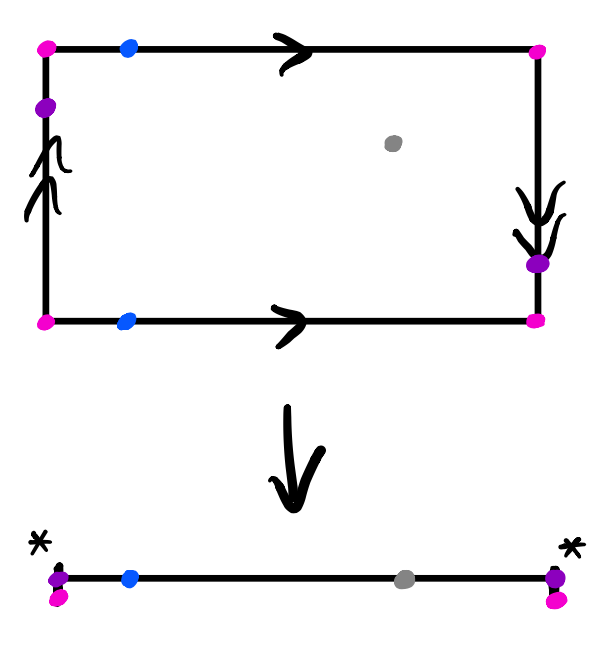
\includegraphics[height=1.35in]{5_3a.png}
\end{center}


\part{}%b
\begin{center}
	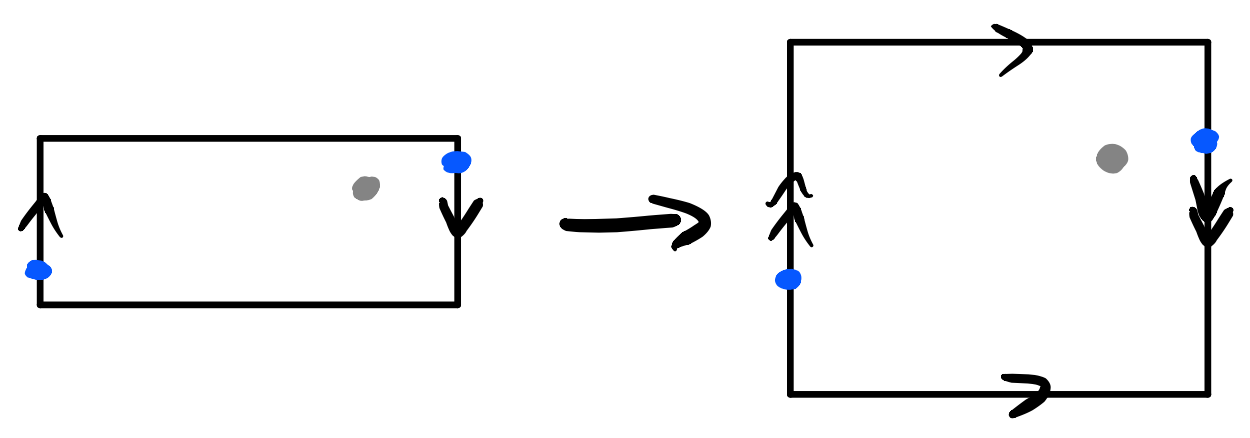
\includegraphics[height=1.05in]{5_3b.png}
\end{center}

\part{}%c
\begin{center}
	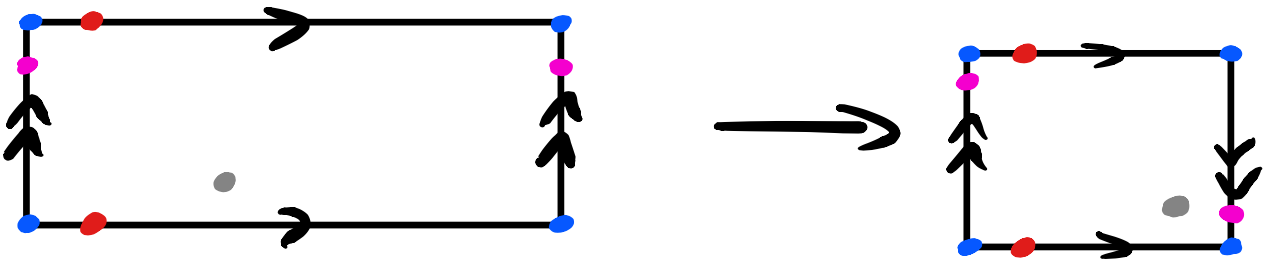
\includegraphics[height=0.65in]{5_3c.png}
\end{center}


\problem{}%4
\begin{enumerate}
	\item Describe the fibers (= pre-images of points) of $g$  in parts (a) and (c).
	\item Prove that in (b),  the closure of the complement of $g(M)$ in $K$  is homeomorphic to $M$.
	
\end{enumerate}
\solution{}
\part{}%a
\noindent
The fibers of $g_1$, the map of the Klein bottle to the circle, are circles on the Klein bottle surface that wrap around the \lq smaller\rq\ axis of the Klein bottle. These circles do not wrap through the \lq mismatched\rq\ identified \lq edge\rq\ of the Klein bottle, although one fiber does exist exactly along this \lq edge of identification\rq. These fibers are drawn in purple on the following diagram.
\begin{center}
	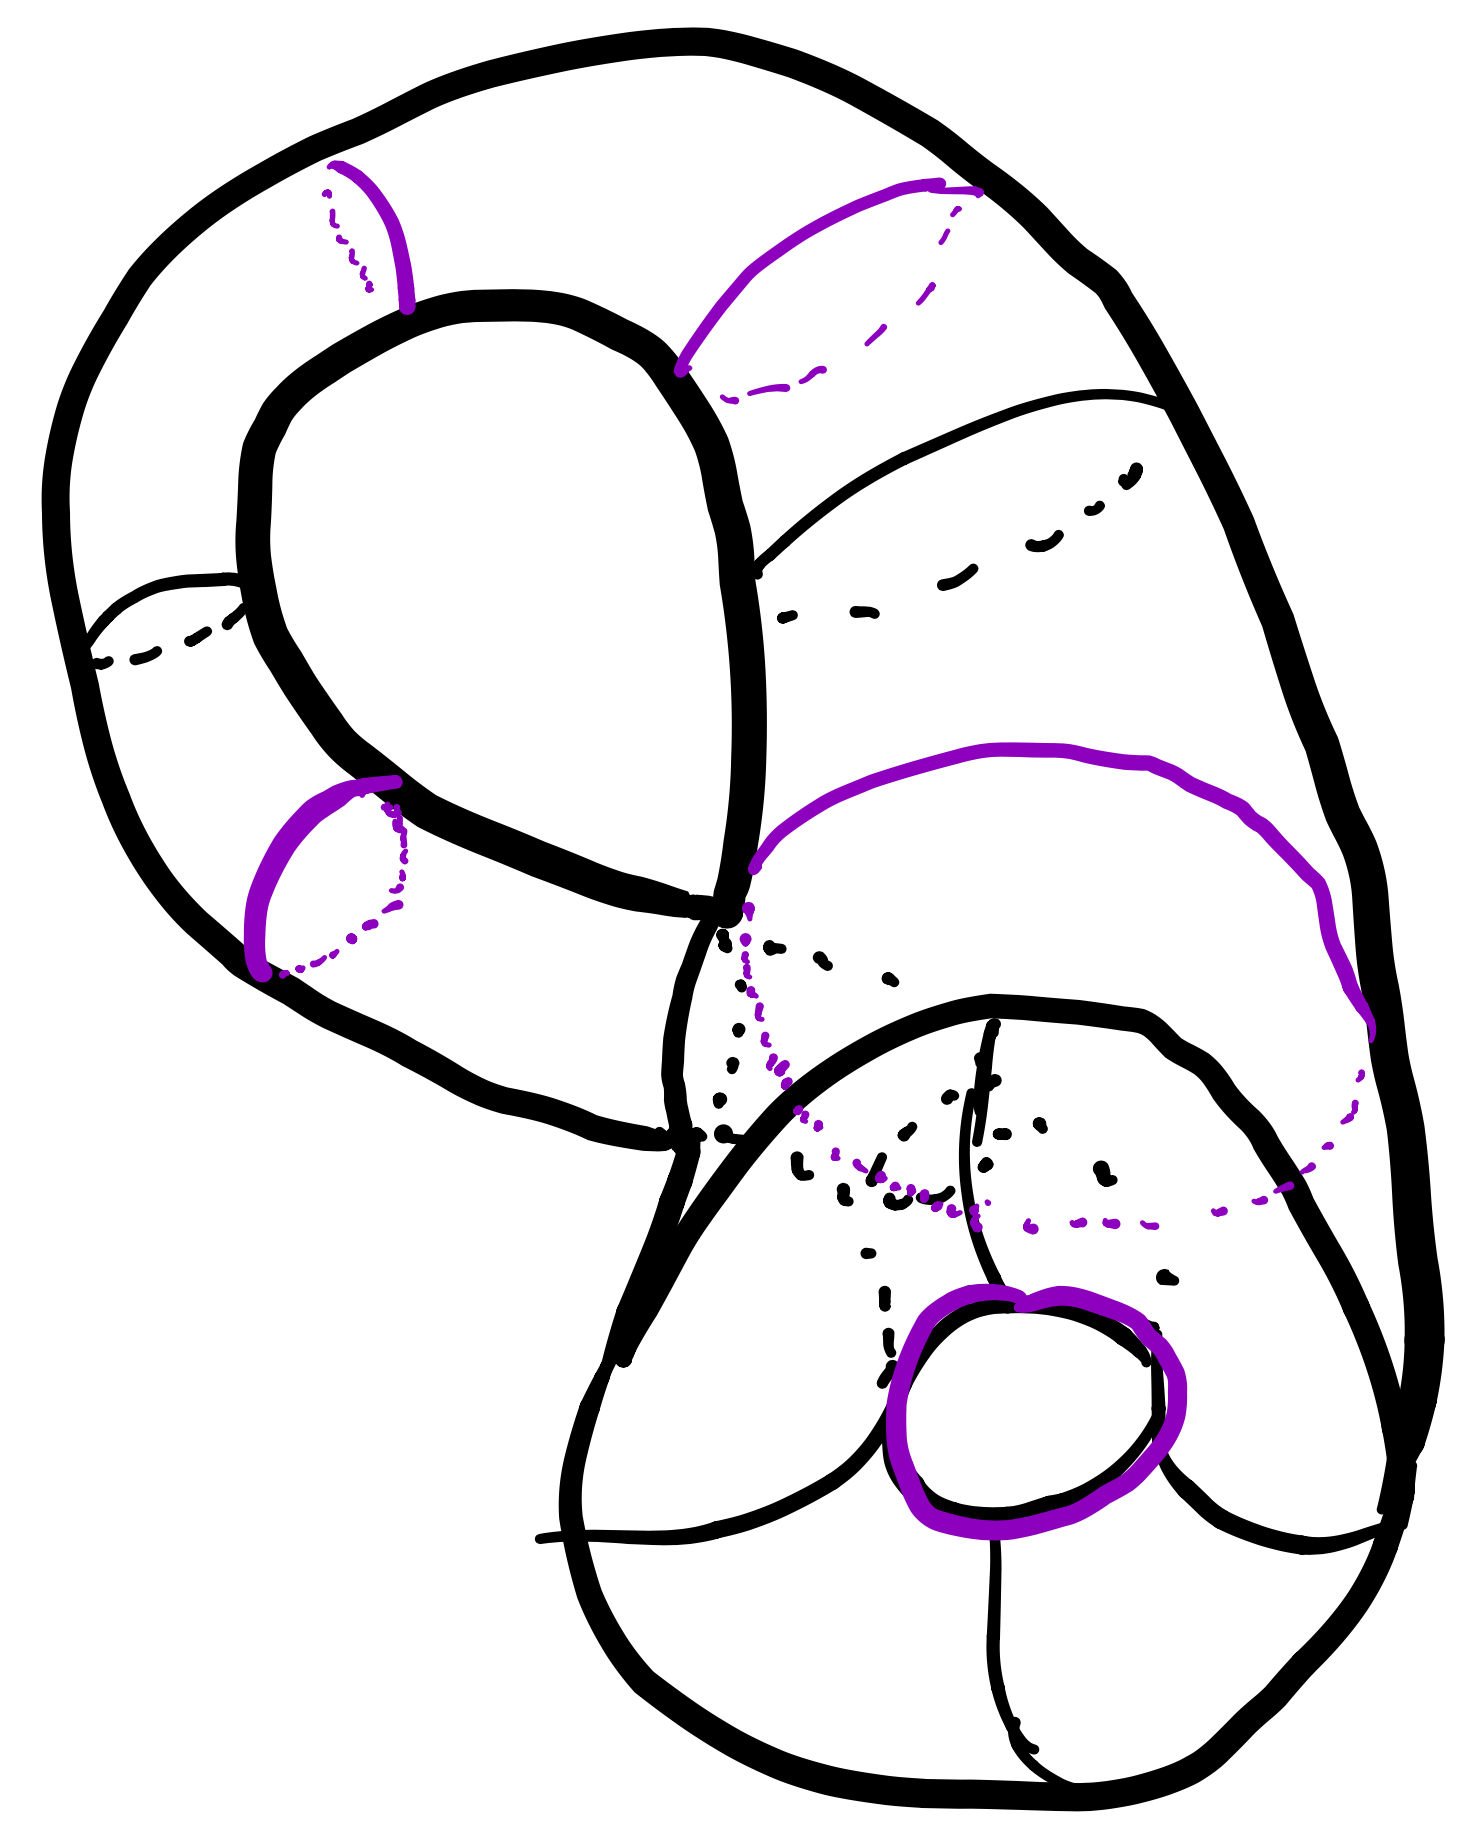
\includegraphics[height=2.2in]{5_4a1.png}
\end{center}


\noindent
The fibers of $g_3$, the map of the Torus to the Klein bottle, are each two points on the torus. These points are equidistant from the upper and lower identified edges in the plane (and equidistant from the horizontal zero) and both shifted an equal amount from zero of 1 in the first dimension. Thus in the torus, these points are radially symmetric but on upper or lower halves of the torus (however this is dependent on the identified edge of the torus being the most outer or inner ring and not on the top, bottom, or anywhere in between). These fibers are drawn in purple and blue in the following diagram. The pink depicts the identified edge.
\begin{center}
	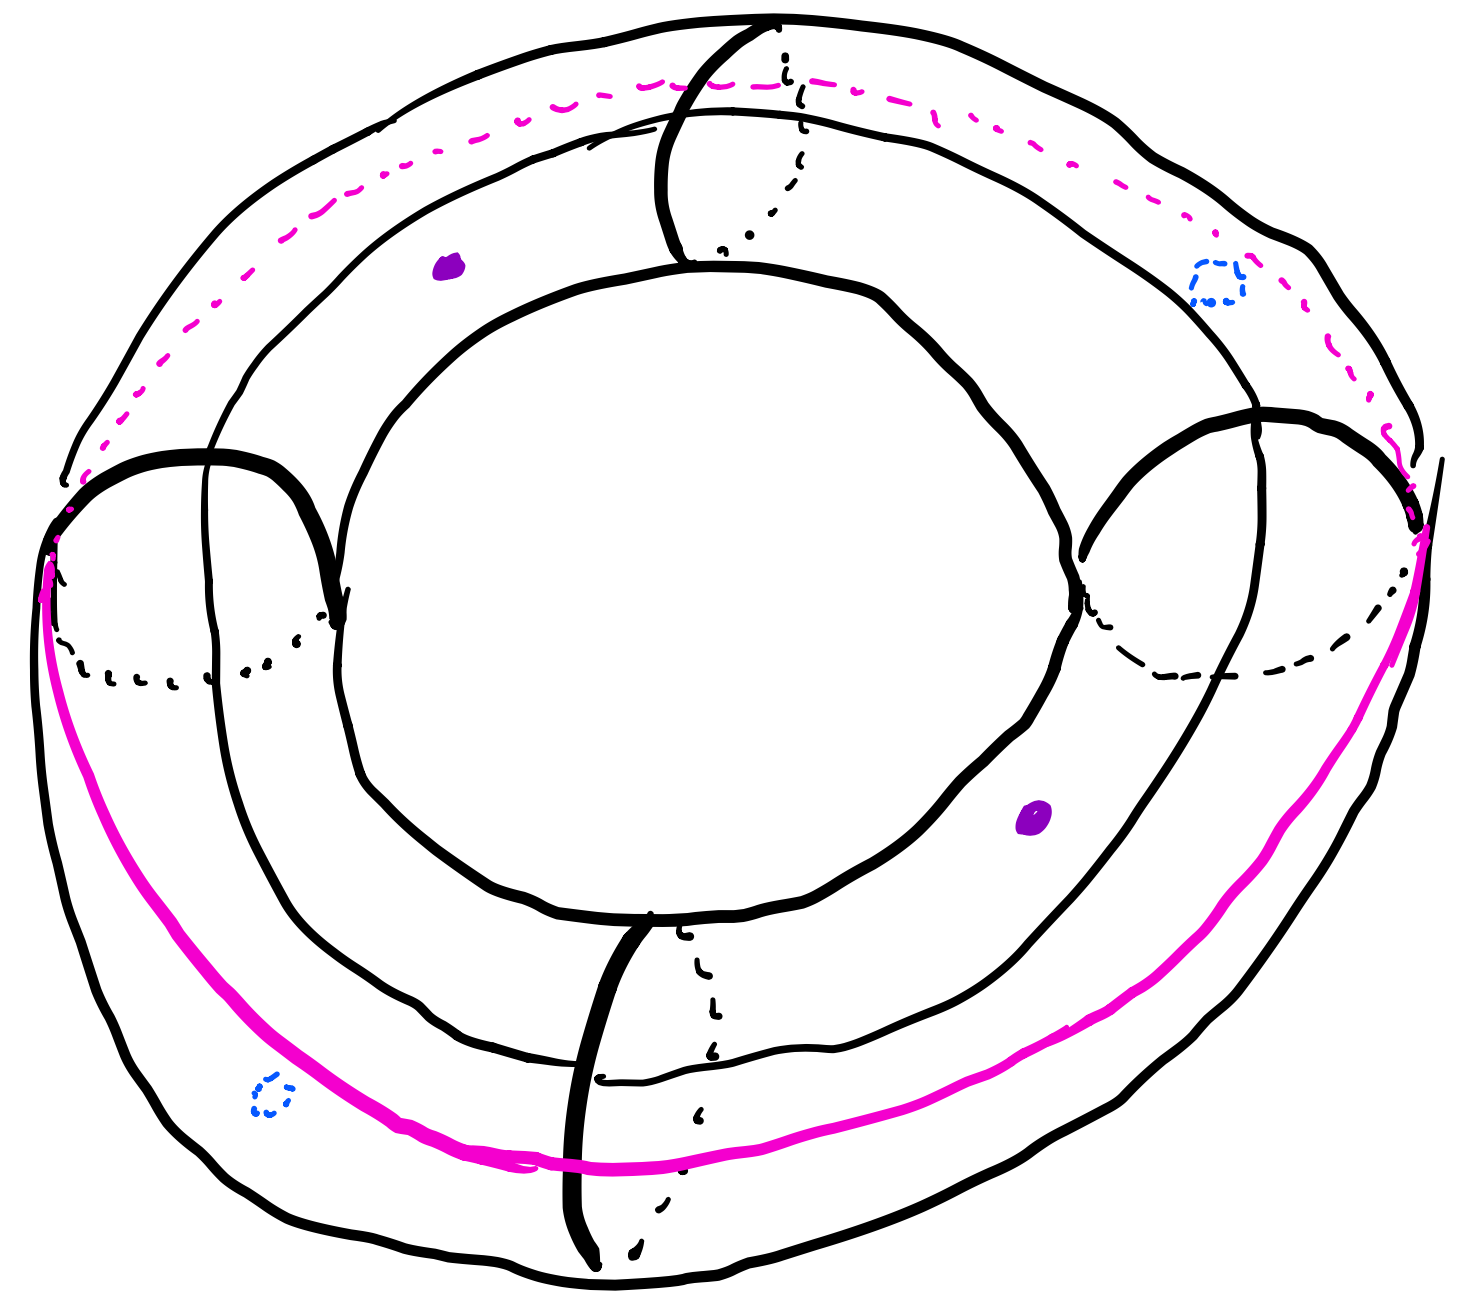
\includegraphics[height=2.2in]{5_4a2.png}
\end{center}

\part{}%b
\noindent The m\"obius strip is shown on the \lq sides\rq\ of the Klein bottle (shaded in gray, bounded by blue), and it complement is the \lq top and bottom\rq\ (shaded in gray in the second panel). The closure ensures that the edges are included in both m\"obius strips. The equivalent depiction of the planar represntation is shown on the next line, with the final panel showing the top and bottom edges being identifications and how they come together to form another m\"obius strip.
\begin{center}
	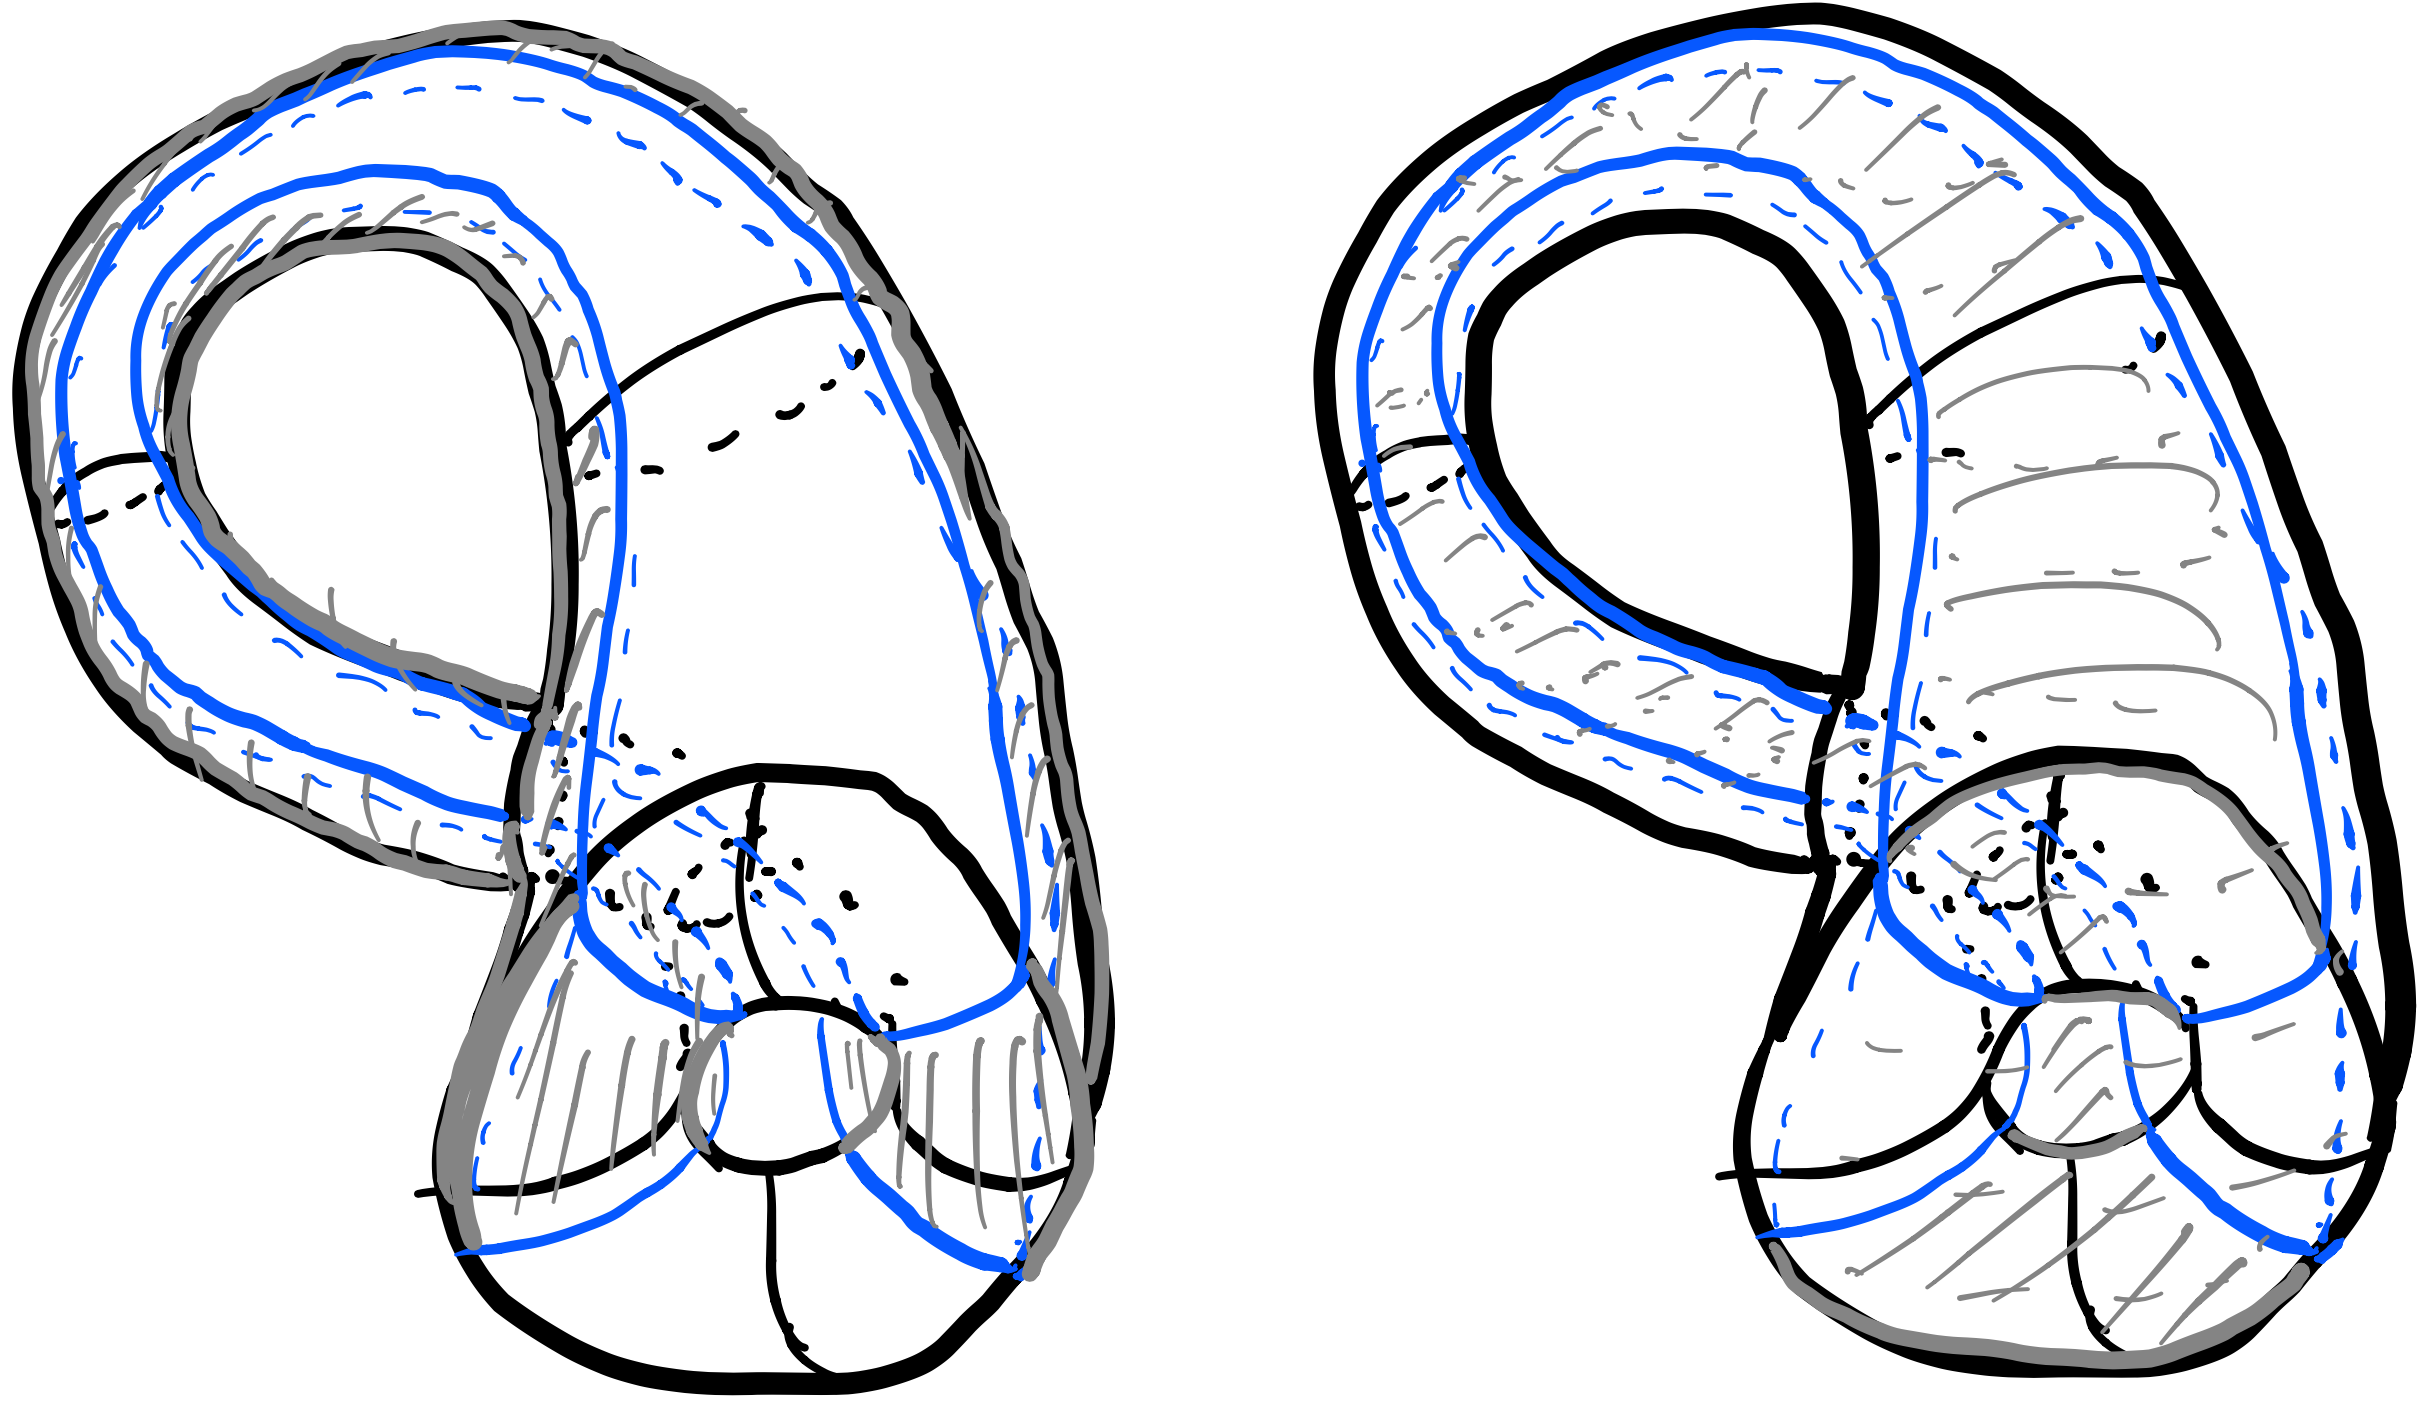
\includegraphics[height=2in]{5_4b1.png}\\
	\vskip 1cm
	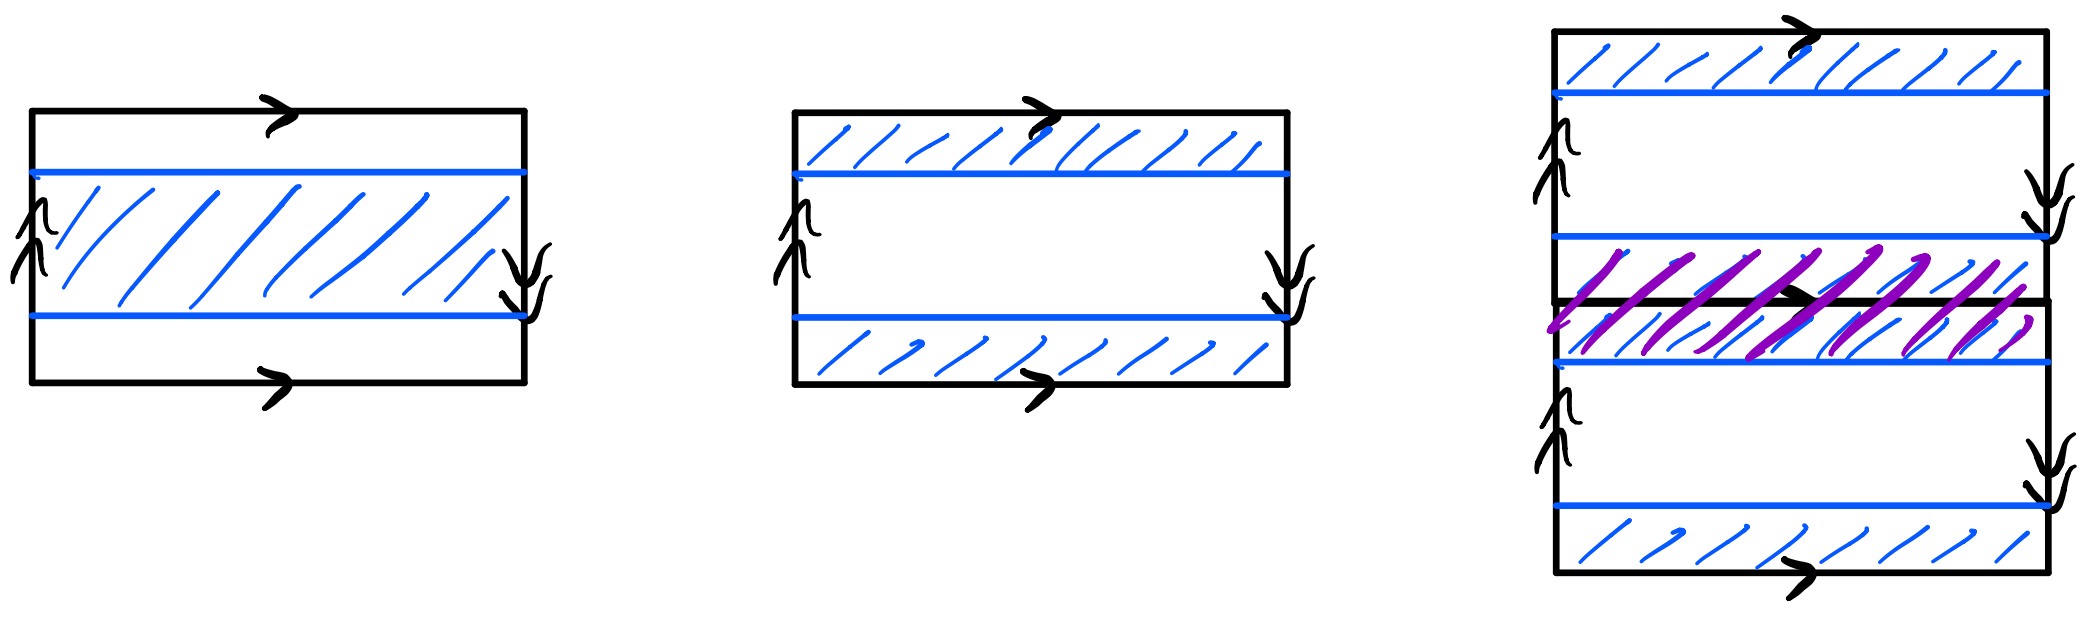
\includegraphics[height=1.5in]{5_4b2.png}
\end{center}



\end{document}